\chapter{Dane i przygotowanie zbioru badawczego}
\label{chap:dane-przygotowanie}

W niniejszym rozdziale opisano proces przygotowania zbioru danych do analizy statystycznej. Jednostką obserwacji w badaniu jest epizod pobytu zwierzęcia w schronisku, rozumiany jako pojedyncze przyjęcie, przypisany do niego wynik kończący pobyt oraz zestaw cech znanych w momencie przyjęcia, czyli cech \emph{intake-time-only}. W rozdziale przedstawiono kolejne etapy przekształcania danych surowych do postaci analitycznej.

\section{Źródło danych i zakres analizy}
\label{sec:zrodlo-danych-zakres}

Materiał empiryczny pochodzi ze schroniska Austin Animal Center (AAC) i został pobrany z bazy Austin Open Data. Baza obejmuje dwie tabele: rejestr przyjęć zwierząt (\emph{intakes}) oraz rejestr wyników kończących pobyt (\emph{outcomes}). Opcjonalnie dane wzbogacono o zmienne kontekstowe, takie jak pogoda.

Zakres czasowy badania obejmuje przyjęcia od 1 października 2013 roku do 4 maja 2025 roku. Analizę ograniczono do psów i kotów, ponieważ stanowią one zasadniczą część populacji schroniskowej. Uwzględnienie rzadziej występujących gatunków, na przykład dzikich zwierząt, mogłoby obniżyć stabilność estymacji.

Wykorzystane dane mają charakter obserwacyjny. Pochodzą z rutynowej dokumentacji schroniska, a nie z kontrolowanego eksperymentu. Z tego powodu analiza obejmuje wyłącznie relacje statystyczne między atrybutami zwierzęcia znanymi w momencie przyjęcia a wynikiem pobytu. Nie formułuje się na tej podstawie wniosków przyczynowo-skutkowych.

\section{Charakterystyka zbiorów wejściowych}
\label{sec:charakterystyka-zbiorow-wejsciowych}

Zbiór analityczny łączy dane o przyjęciu z danymi o wyniku końcowym. Rozdzielenie tych warstw na etapie modelowania pozwala ograniczyć ryzyko wykorzystania informacji z przyszłości, czyli wycieku danych.

\begin{table}[htbp]
\centering
\caption{Porównanie dwóch podstawowych zbiorów wejściowych}
\label{tab:porownanie-zbiorow-wejsciowych}
\small
\begin{tabular}{|p{0.18\textwidth}|p{0.53\textwidth}|p{0.19\textwidth}|}
\hline
\rowcolor{LightGray}
\textbf{Warstwa danych} & \textbf{Przykładowe pola kluczowe} & \textbf{Rola w procesie} \\
\hline
Rejestr przyjęć & \texttt{animal\_id}, \texttt{animal\_type}, \texttt{intake\_datetime}, \texttt{intake\_type}, \texttt{intake\_condition}, \texttt{sex\_upon\_intake}, \texttt{age\_upon\_intake}, \texttt{breed}, \texttt{color} & Źródło atrybutów wejściowych ($X$) \\
\hline
Rejestr wyników & \texttt{animal\_id}, \texttt{animal\_type}, \texttt{outcome\_datetime}, \texttt{outcome\_type}, \texttt{outcome\_subtype}, \texttt{sex\_upon\_outcome} & Źródło zmiennej docelowej ($y$) \\
\hline
\end{tabular}
\end{table}

Metadane generowane na końcu pobytu, takie jak \texttt{outcome\_type} i \texttt{outcome\_datetime}, wyodrębniono jako zmienne docelowe. Podział ten zapisano w oddzielnych plikach konfiguracyjnych JSON dla cech oraz targetów.

\section{Standaryzacja i czyszczenie danych}
\label{sec:standaryzacja-czyszczenie}

Czyszczenie danych przeprowadzono ostrożnie, bez sztucznej imputacji braków. Nazwy zmiennych zapisano w formacie \texttt{snake\_case}. Daty ujednolicono do lokalnej strefy czasowej schroniska, konwertując ciągi znaków do formatu \texttt{datetime64}.

Sprawdzono kompletność kluczowych atrybutów: \texttt{animal\_id}, \texttt{animal\_type}, \texttt{intake\_datetime}, \texttt{outcome\_datetime} oraz \texttt{outcome\_type}. Obserwacje z brakami w tych polach usunięto. Dokładne duplikaty rekordów zostały odfiltrowane.

\begin{table}[htbp]
\centering
\caption{Redukcja liczby rekordów w kolejnych etapach budowy zbioru modelowego}
\label{tab:atrycja-danych}
\footnotesize
\begin{tabular}{|p{0.46\textwidth}|>{\raggedleft\arraybackslash}p{0.18\textwidth}|>{\raggedleft\arraybackslash}p{0.18\textwidth}|}
\hline
\rowcolor{LightGray}
\textbf{Zbiór danych na danym etapie} & \textbf{Liczba wierszy} & \textbf{Liczba usuniętych} \\
\hline
Zbiór źródłowy wejść (\texttt{intakes.csv}) & 173 812 & --- \\
\hline
Zbiór źródłowy wyjść (\texttt{outcomes.csv}) & 173 775 & --- \\
\hline
Standaryzacja i filtracja wejść & 163 901 & 9 911 \\
\hline
Standaryzacja i filtracja wyjść & 163 880 & 9 895 \\
\hline
Dopasowane epizody z targetem & 162 390 & 1 511 \\
\hline
Finalny zbiór modelowy & 162 390 & 0 \\
\hline
\end{tabular}
\end{table}

Większość usuniętych rekordów dotyczyła zwierząt innych niż psy i koty. Usunięto również 1 511 przyjęć pozbawionych chronologicznie poprawnego wyniku końcowego. W modelowaniu nadzorowanym potraktowano je jako obserwacje bez dostępnej etykiety docelowej i wykluczono z finalnego zbioru; w ujęciu analizy przeżycia mogłyby być one rozważane jako obserwacje cenzorowane. Brakujące dane w atrybutach predykcyjnych występowały pojedynczo: odnotowano 9 braków wieku i 1 brak płci.

\section{Konstrukcja epizodów i dopasowanie rekordów}
\label{sec:konstrukcja-epizodow}

Jednostką analizy jest epizod pobytu. Ponieważ to samo zwierzę (\texttt{animal\_id}) może być kilkukrotnie rejestrowane w schronisku, każde przyjęcie połączono z najbliższym w czasie, niewykorzystanym wcześniej wynikiem. Zastosowano więc metodę najbliższego wolnego zdarzenia w czasie, aby odtworzyć możliwie spójną historię pobytu.

Taka procedura zapobiega powstawaniu ujemnych czasów pobytu oraz wielokrotnemu przypisaniu tego samego wyniku do różnych przyjęć. Audyt zbioru potwierdził poprawność łączenia --- nie odnotowano epizodów nakładających się w czasie.

\begin{figure}[htbp]
\centering
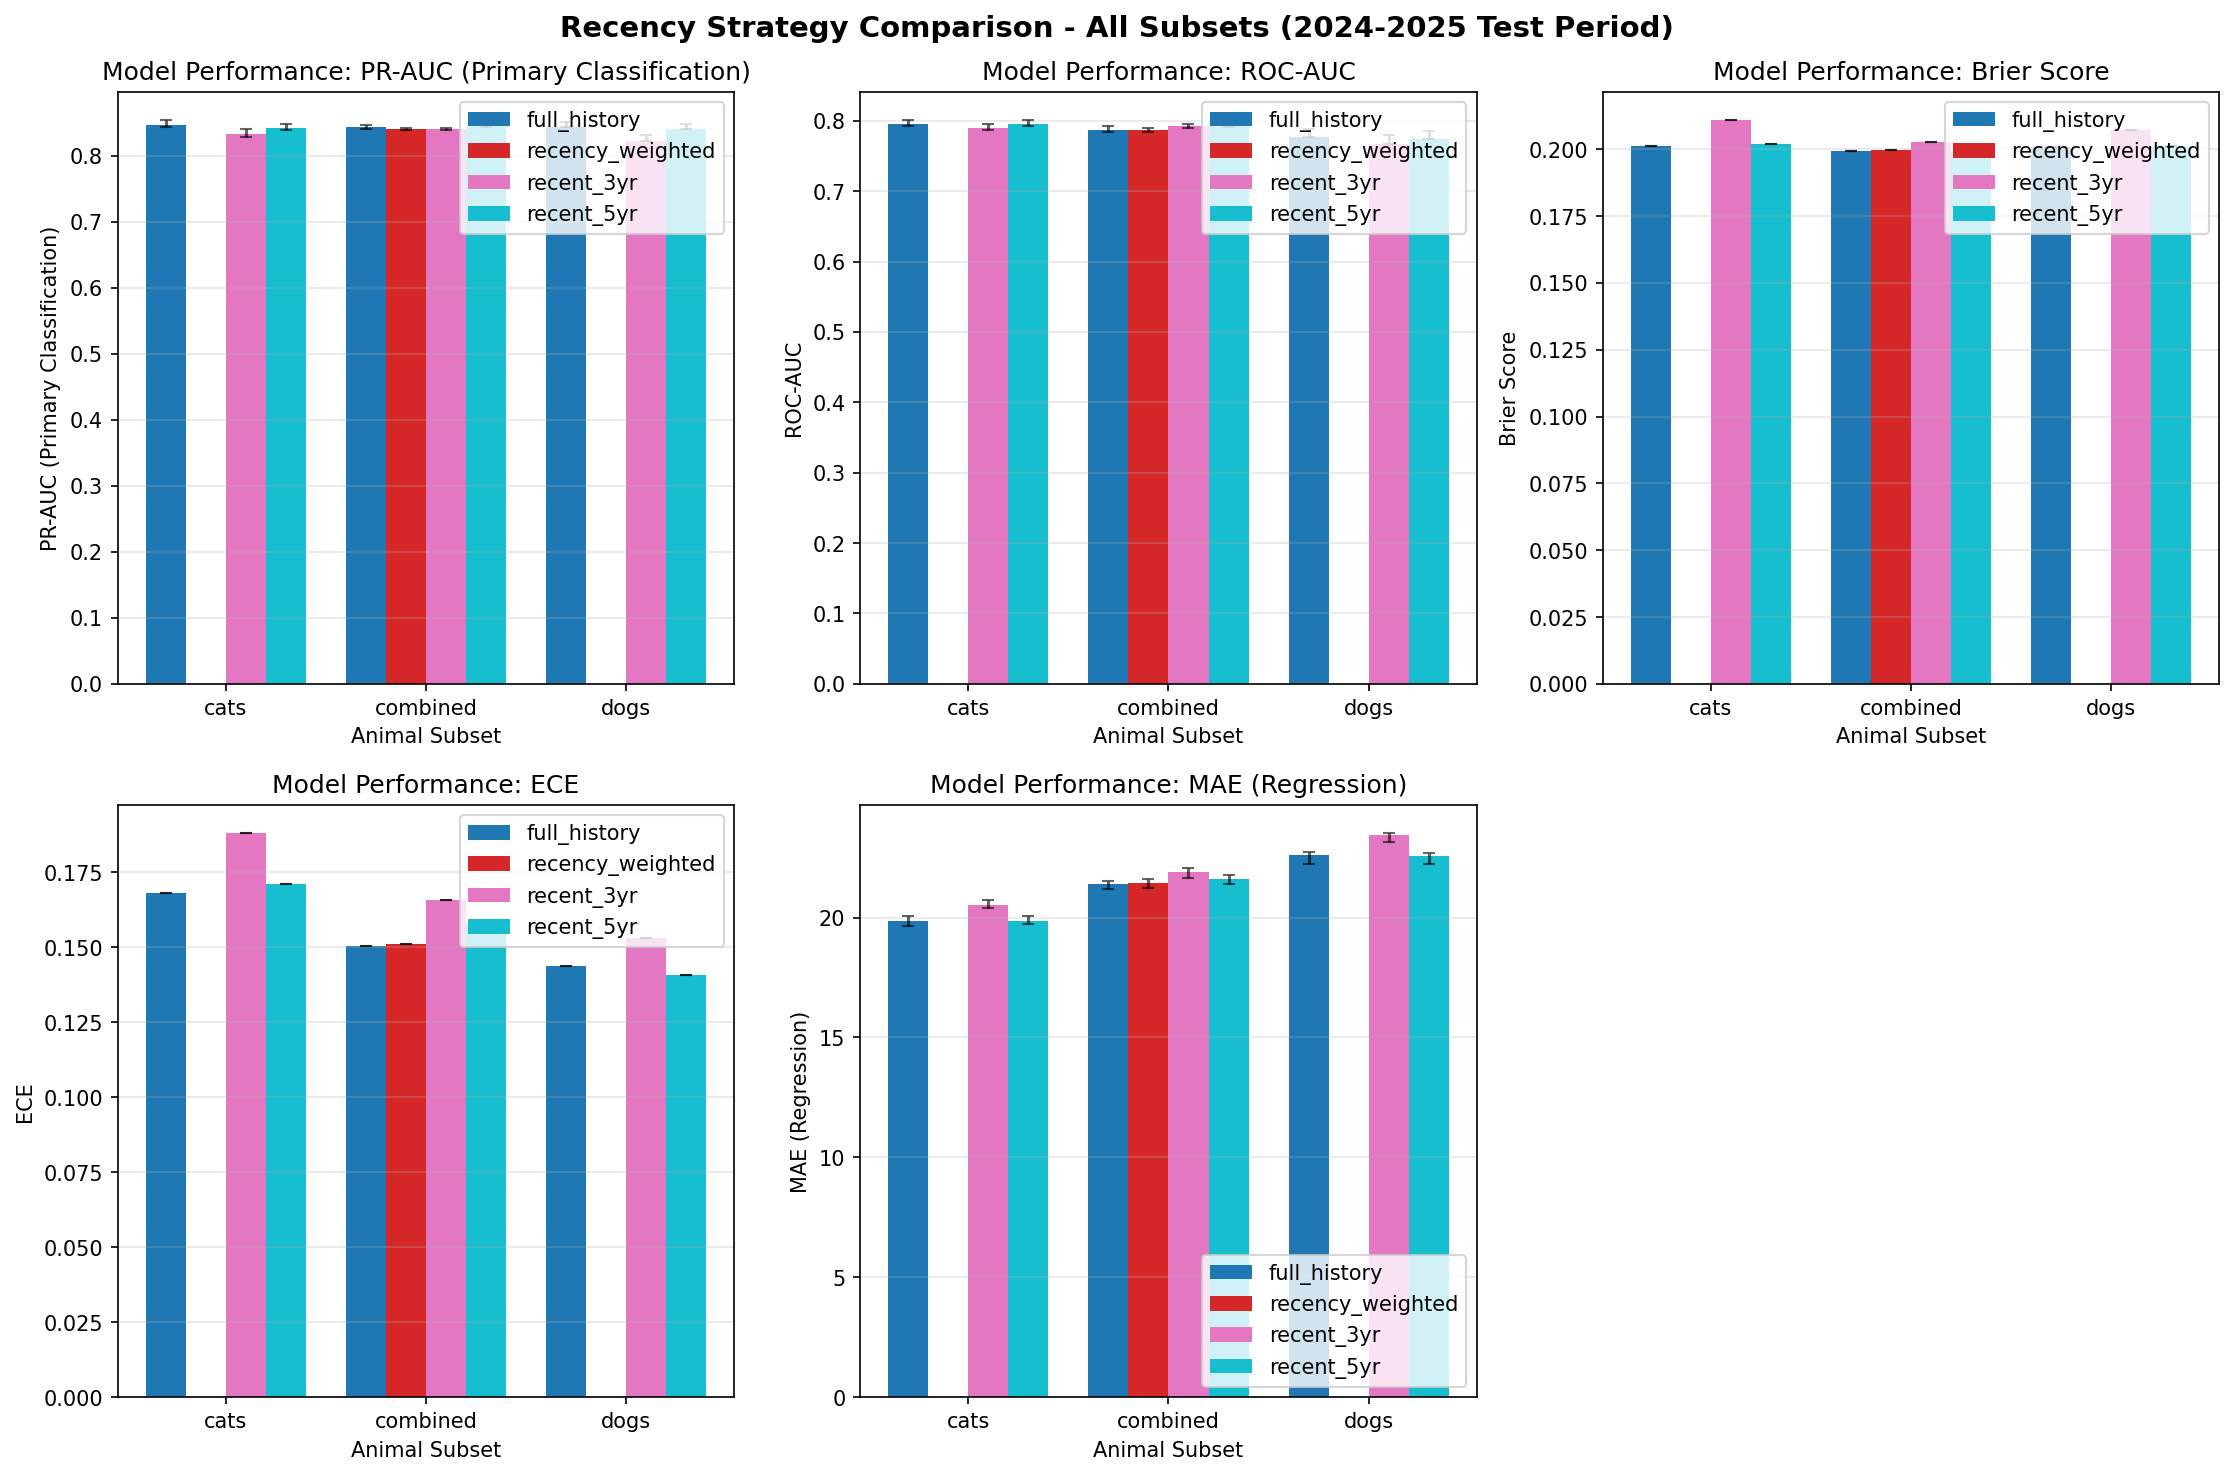
\includegraphics[width=0.92\textwidth]{../reports/figures/recency_strategy_comparison.png}
\caption{Porównanie strategii dopasowania rekordów przyjęcia i wyniku.}
\label{fig:recency_strategy}
\end{figure}

\section{Zmienne docelowe}
\label{sec:zmienne-docelowe}

Zdefiniowano dwie główne zmienne docelowe przeznaczone do późniejszego modelowania:

\begin{table}[htbp]
\centering
\caption{Formalne definicje zmiennych docelowych}
\label{tab:definicje-zmiennych-docelowych}
\scriptsize
\begin{tabular}{|p{0.37\textwidth}|p{0.30\textwidth}|p{0.23\textwidth}|}
\hline
\rowcolor{LightGray}
\textbf{Zmienna} & \textbf{Definicja} & \textbf{Interpretacja} \\
\hline
\texttt{classification\_target} & 1 dla \texttt{Adoption}, 0 dla innych & Binarny wynik adopcji \\
\hline
\texttt{regression\_target\_days} & $(\textit{outcome\_time} - \textit{intake\_time}) \div 86400$ & Długość pobytu do dowolnego wyniku (adopcja, transfer, eutanazja lub zgon) \\
\hline
\texttt{days\_to\_adoption} & Wartość \texttt{regression\_target\_days} dla adoptowanych & Stosowana wyłącznie w opisowej analizie czasu oczekiwania (nie jako cel modelowania regresji) \\
\hline
\end{tabular}
\end{table}

Adopcją zakończyło się 50,87\% uwzględnionych epizodów, czyli 82 609 przypadków. Pozostałe 49,13\% obejmuje powroty do właściciela, transfery, eutanazję oraz zgony. Czas do dowolnego zdarzenia potraktowano jako klasyczny problem regresji, ponieważ długość zajmowania boksu przekłada się bezpośrednio na koszty operacyjne placówki.

\section{Konstrukcja cech wejściowych}
\label{sec:konstrukcja-cech-wejsciowych}

Cechy wejściowe zbudowano wyłącznie na podstawie informacji dostępnych w chwili przyjęcia.

\begin{table}[htbp]
\centering
\caption{Grupy cech wejściowych}
\label{tab:grupy-cech-wejsciowych}
\small
\begin{tabular}{|p{0.28\textwidth}|p{0.62\textwidth}|}
\hline
\rowcolor{LightGray}
\textbf{Grupa} & \textbf{Zmienne} \\
\hline
Cechy ogólne & \texttt{animal\_type}, \texttt{sex\_upon\_intake}, \texttt{intake\_condition} \\
\hline
Wiek & \texttt{age\_days}, \texttt{age\_years}, \texttt{age\_group} (np. \texttt{baby}, \texttt{senior}) \\
\hline
Rasa & \texttt{breed}, \texttt{primary\_breed}, \texttt{simplified\_breed\_group} \\
\hline
Umaszczenie & \texttt{color}, \texttt{primary\_color}, \texttt{simplified\_color\_group} \\
\hline
Kontekst przyjęcia & \texttt{intake\_season}, \texttt{intake\_type}, \texttt{covid\_period} \\
\hline
Cechy binarne & \texttt{has\_name}, \texttt{is\_mixed\_breed}, \texttt{is\_black\_or\_dark} \\
\hline
Cechy czasowe & \texttt{intake\_month}, \texttt{intake\_year}, \texttt{intake\_season} \\
\hline
\end{tabular}
\end{table}

Aby ograniczyć liczbę kategorii, rasy i umaszczenia pogrupowano w szersze klasy, takie jak \texttt{pit\_bull\_type}, \texttt{terrier\_type} czy \texttt{domestic\_cat}. Oryginalna zmienna opisująca rasę zawierała 2 761 unikalnych wartości, z których większość występowała bardzo rzadko.

Na podstawie daty przyjęcia zdefiniowano okresy związane z pandemią: przed COVID-19, czyli do 1 marca 2020 r.; w trakcie pandemii, od marca 2020 do grudnia 2021; oraz po pandemii, od 1 stycznia 2022 r. Wiek przekształcono z wartości tekstowych, na przykład \texttt{2 years}, do postaci w pełni numerycznej w dniach oraz do kategorii wiekowych.

Cechy wejściowe przebadano pod kątem multikolinearności za pomocą wskaźnika VIF (ang. \emph{Variance Inflation Factor}). Za próg krytyczny przyjęto $\text{VIF} > 10$. Analiza wykazała krytyczną redundancję pomiędzy wariantami reprezentacji wieku: \texttt{age\_days} uzyskał wartość VIF~=~2971, a \texttt{age\_group\_senior} --- VIF~=~4341. Warianty liniowo zależne od siebie zredukowano do jednej numerycznej reprezentacji. Modele drzewiaste są odporne na multikolinearność, jednak ograniczenie redundancji zmniejsza przestrzeń cech i przyspiesza uczenie.

\section{Charakterystyka opisowa zbioru}
\label{sec:charakterystyka-opisowa-zbioru}

Zbiór obejmujący 162 390 pobytów pozwala przedstawić podstawowe statystyki opisowe. Najważniejsze wskaźniki zmieniały się w czasie:

\begin{figure}[htbp]
\centering
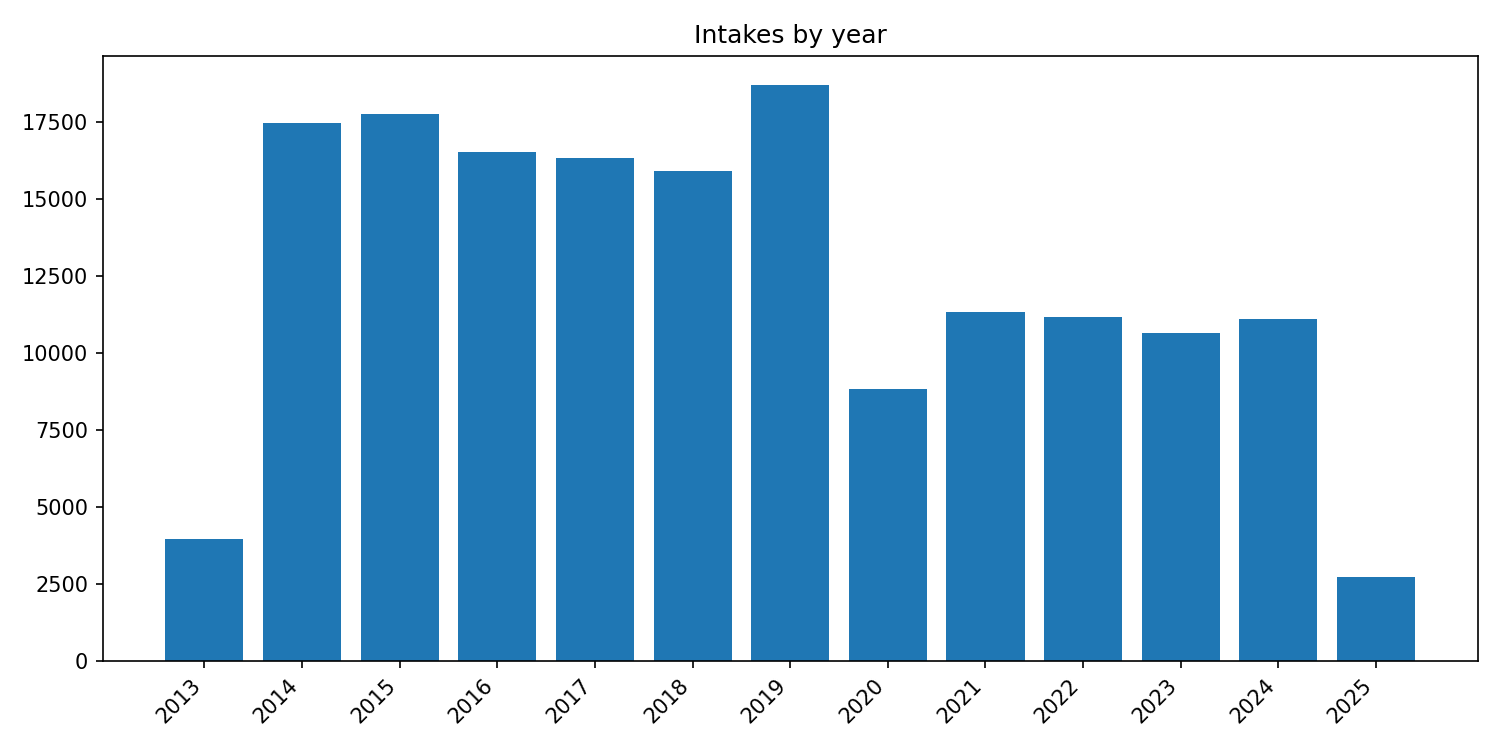
\includegraphics[width=0.92\textwidth]{../reports/figures/intakes_by_year.png}
\caption{Roczna liczba przyjęć zwierząt do Austin Animal Center w latach 2013--2025.}
\label{fig:intakes_by_year}
\end{figure}

\begin{figure}[htbp]
\centering
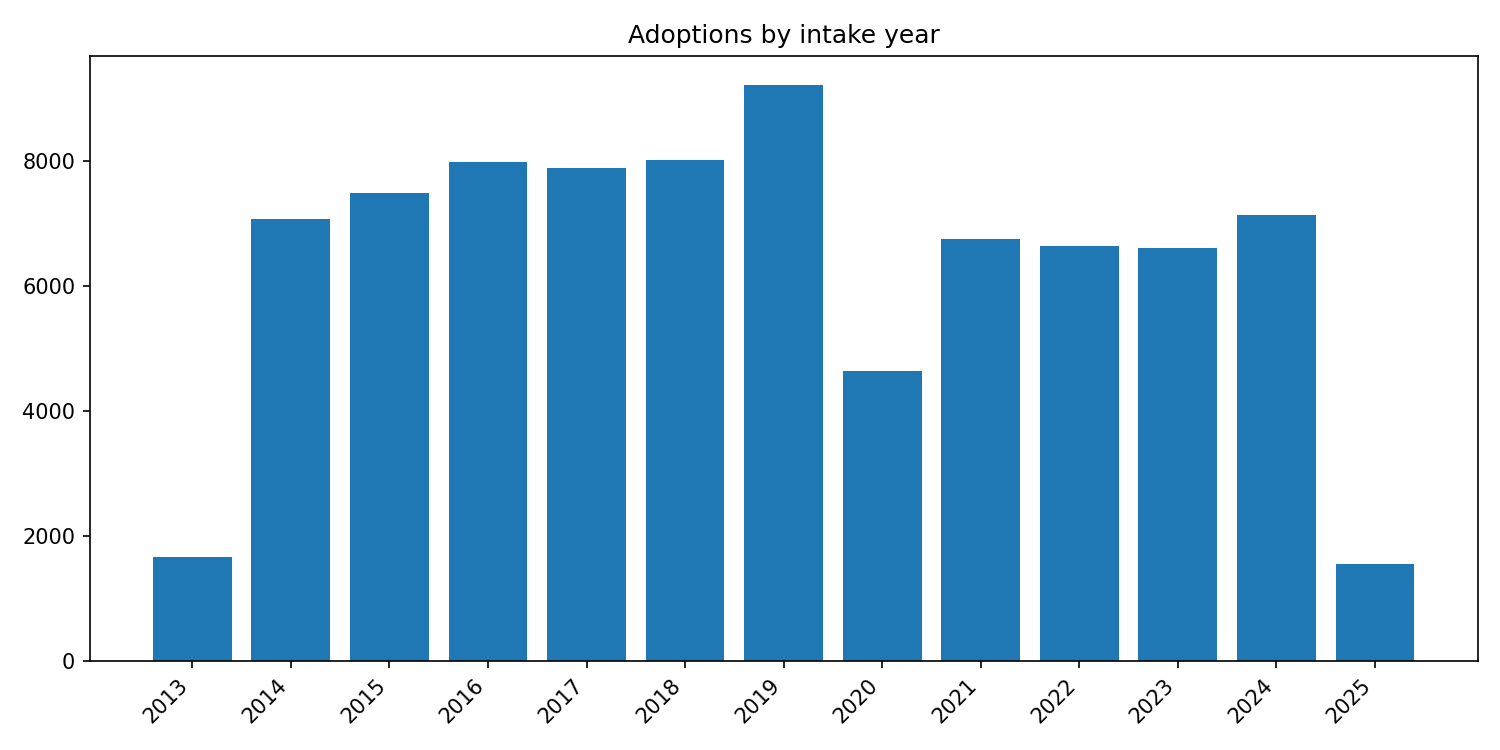
\includegraphics[width=0.92\textwidth]{../reports/figures/adoptions_by_year.png}
\caption{Roczna liczba adopcji w Austin Animal Center.}
\label{fig:adoptions_by_year}
\end{figure}

\begin{itemize}\itemsep2pt
\item \textbf{Przed COVID-19 (108~785 epizodów):} wskaźnik adopcji wynosił 46,3\%, a mediana całkowitej długości pobytu, liczona dla każdego wyniku, była równa 5,25 dnia.
\item \textbf{COVID-19 (17~946 epizodów):} wskaźnik adopcji wzrósł do 57,2\%, a mediana pobytu do 8,01 dnia.
\item \textbf{Post COVID-19 (35~624 epizodów):} wskaźnik adopcji wyniósł 61,5\%, a mediana pobytu 9,83 dnia.
\end{itemize}

Zmiany te zbiegają się ze zmianą struktury przyjmowanych zwierząt. Odsetek psów spadł z 60,45\% w okresie przedpandemicznym do 50,65\%. Jednocześnie odsetek młodych zwierząt (\texttt{baby}) wzrósł z 44,11\% do 54,34\%.

Psy i koty różnią się pod względem dynamiki adopcji. Ogólny wskaźnik adopcji był zbliżony dla obu grup: 50,28\% dla psów i 51,68\% dla kotów. Wśród zwierząt adoptowanych do 30 dni schronisko opuszcza jednak 73,6\% psów i 54,5\% kotów.

\begin{figure}[htbp]
\centering
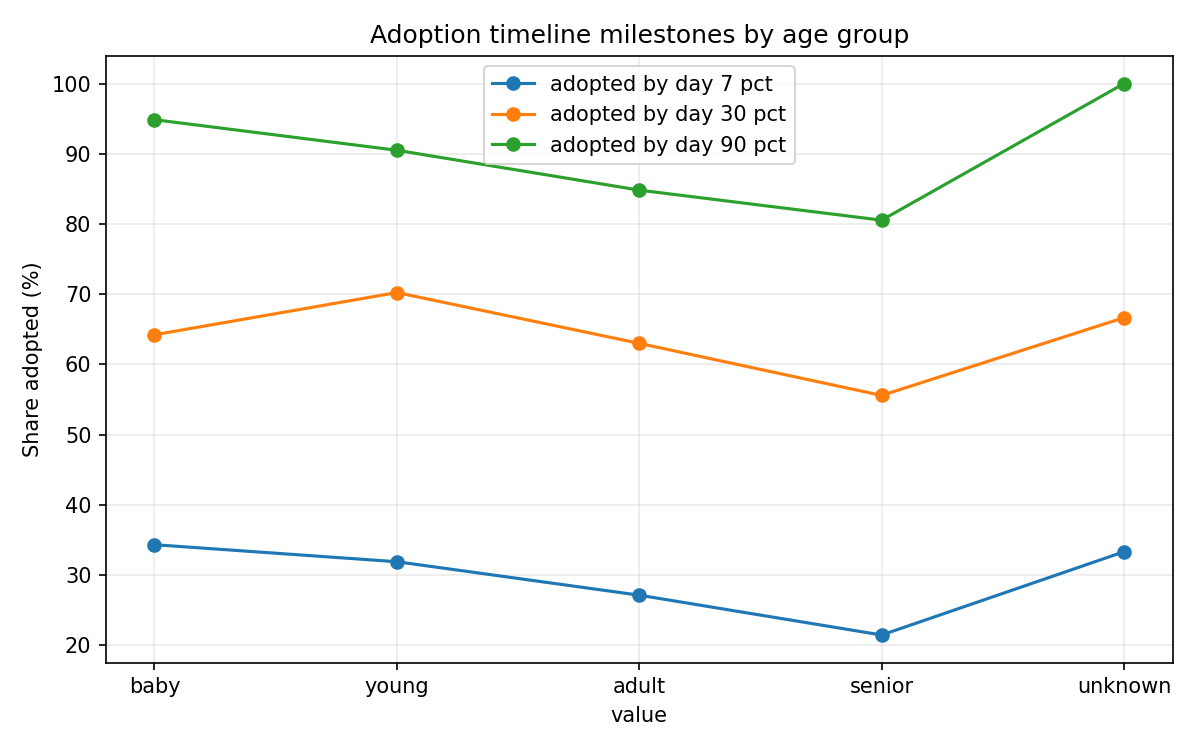
\includegraphics[width=0.92\textwidth]{../reports/figures/adoption_cumulative_curves.png}
\caption{Skumulowane krzywe adopcji dla psów i kotów.}
\label{fig:adoption_cumulative_curves}
\end{figure}

\begin{figure}[htbp]
\centering
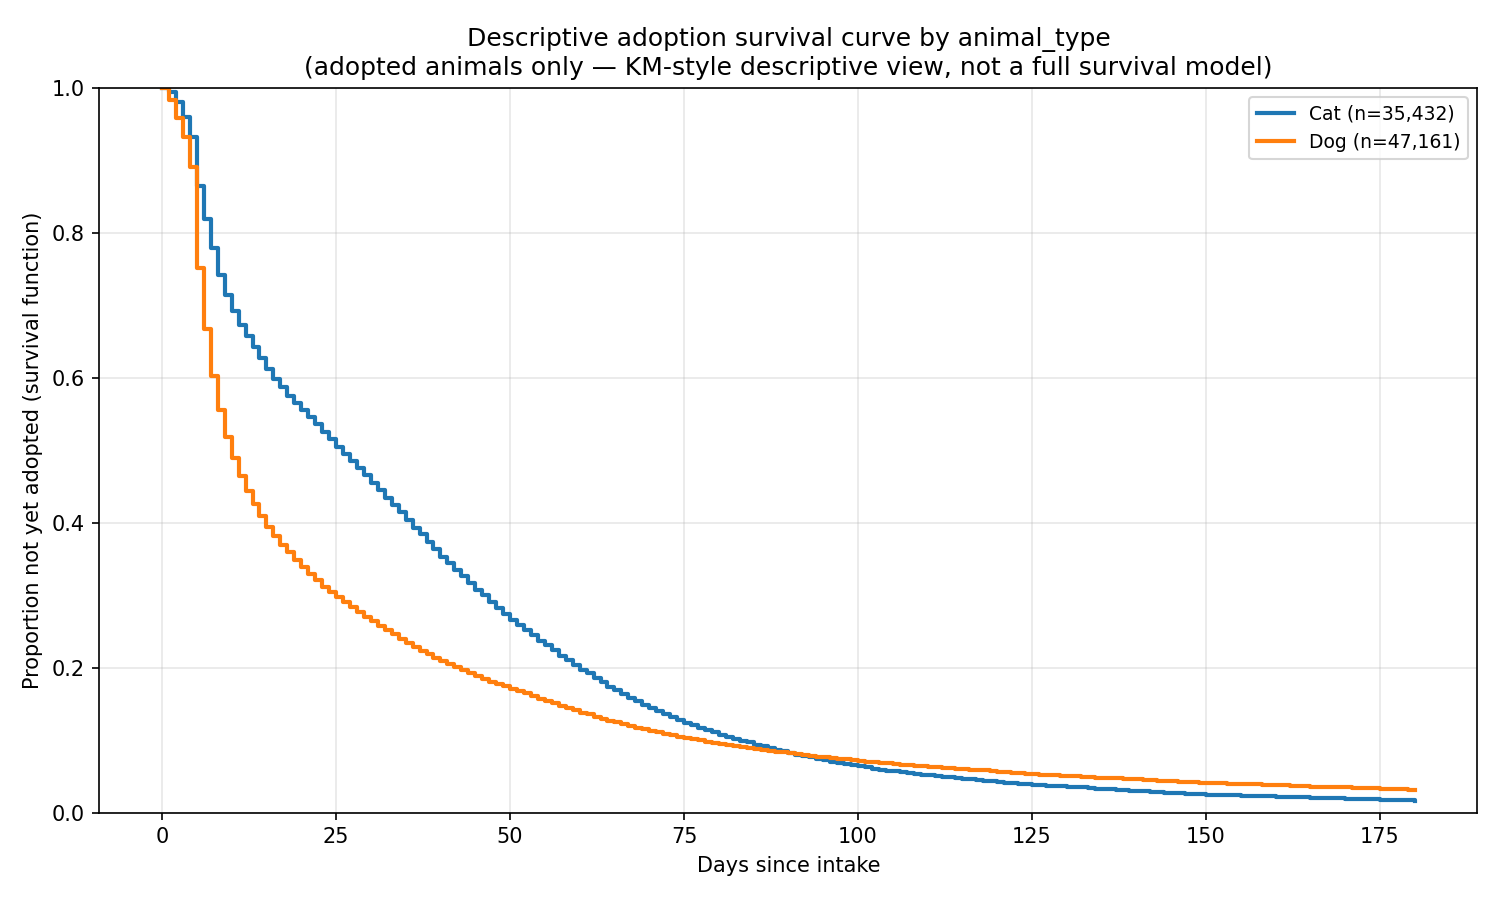
\includegraphics[width=0.92\textwidth]{../reports/figures/km_adoption_by_animal_type.png}
\caption{Krzywe Kaplana-Meiera prawdopodobieństwa adopcji w funkcji czasu pobytu, z podziałem na psy i koty.}
\label{fig:km_adoption}
\end{figure}

\begin{figure}[htbp]
\centering
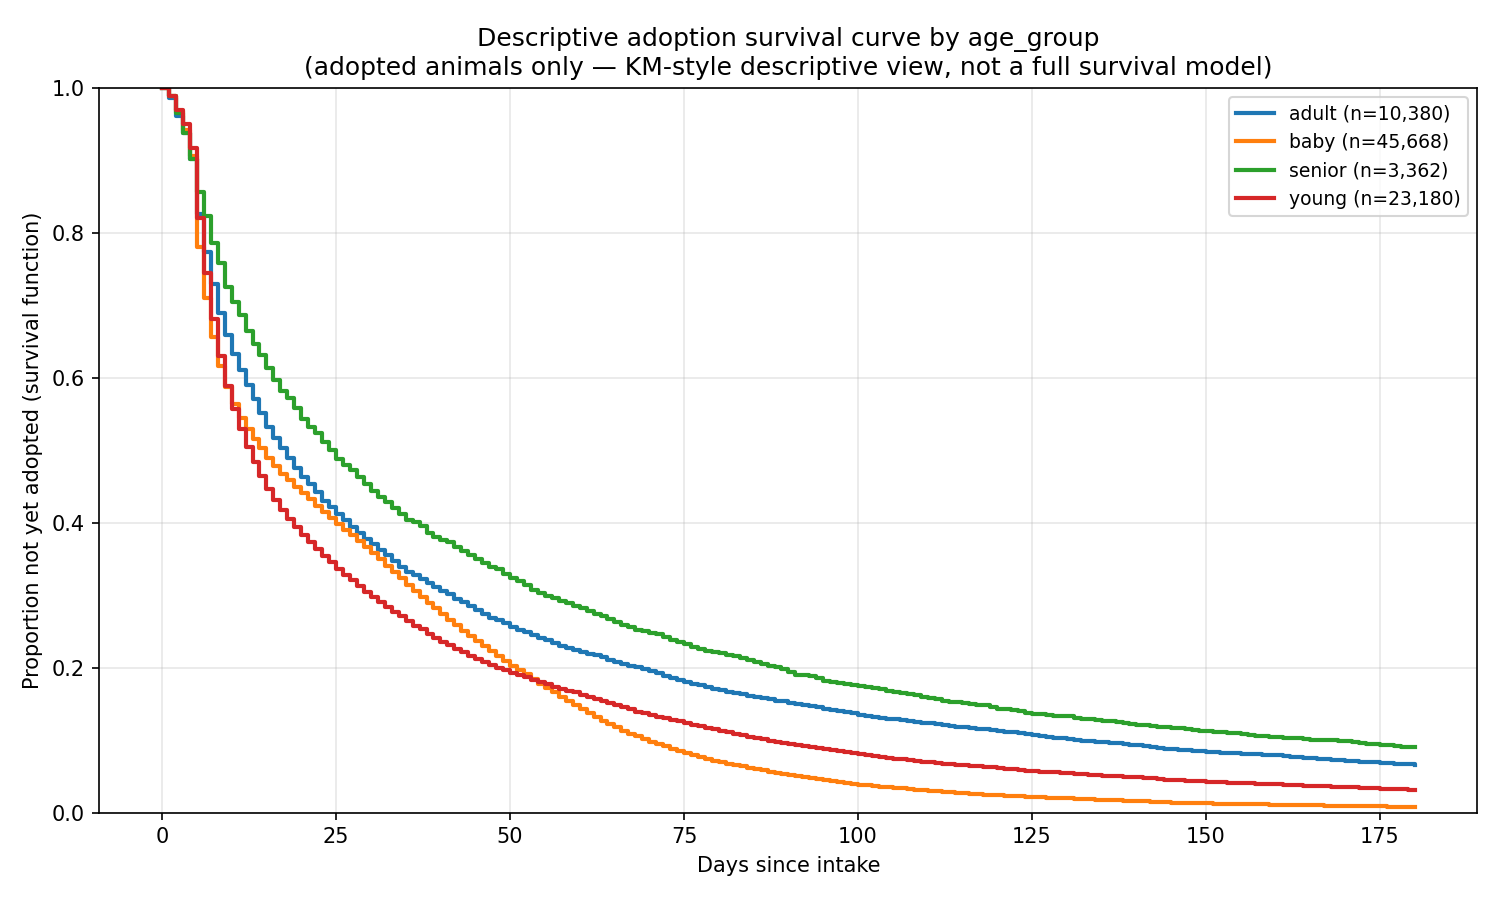
\includegraphics[width=0.92\textwidth]{../reports/figures/km_adoption_by_age_group.png}
\caption{Krzywe Kaplana-Meiera czasu do adopcji w podziale na grupy wiekowe zwierzęcia (wyłącznie adoptowane). Zwierzęta z grupy \texttt{baby} opuszczają schronisko najszybciej; krzywa dla grupy \texttt{senior} opada wolniej i osiąga niższy poziom skumulowanej adopcji.}
\label{fig:km_adoption_by_age_group}
\end{figure}

\begin{figure}[htbp]
\centering
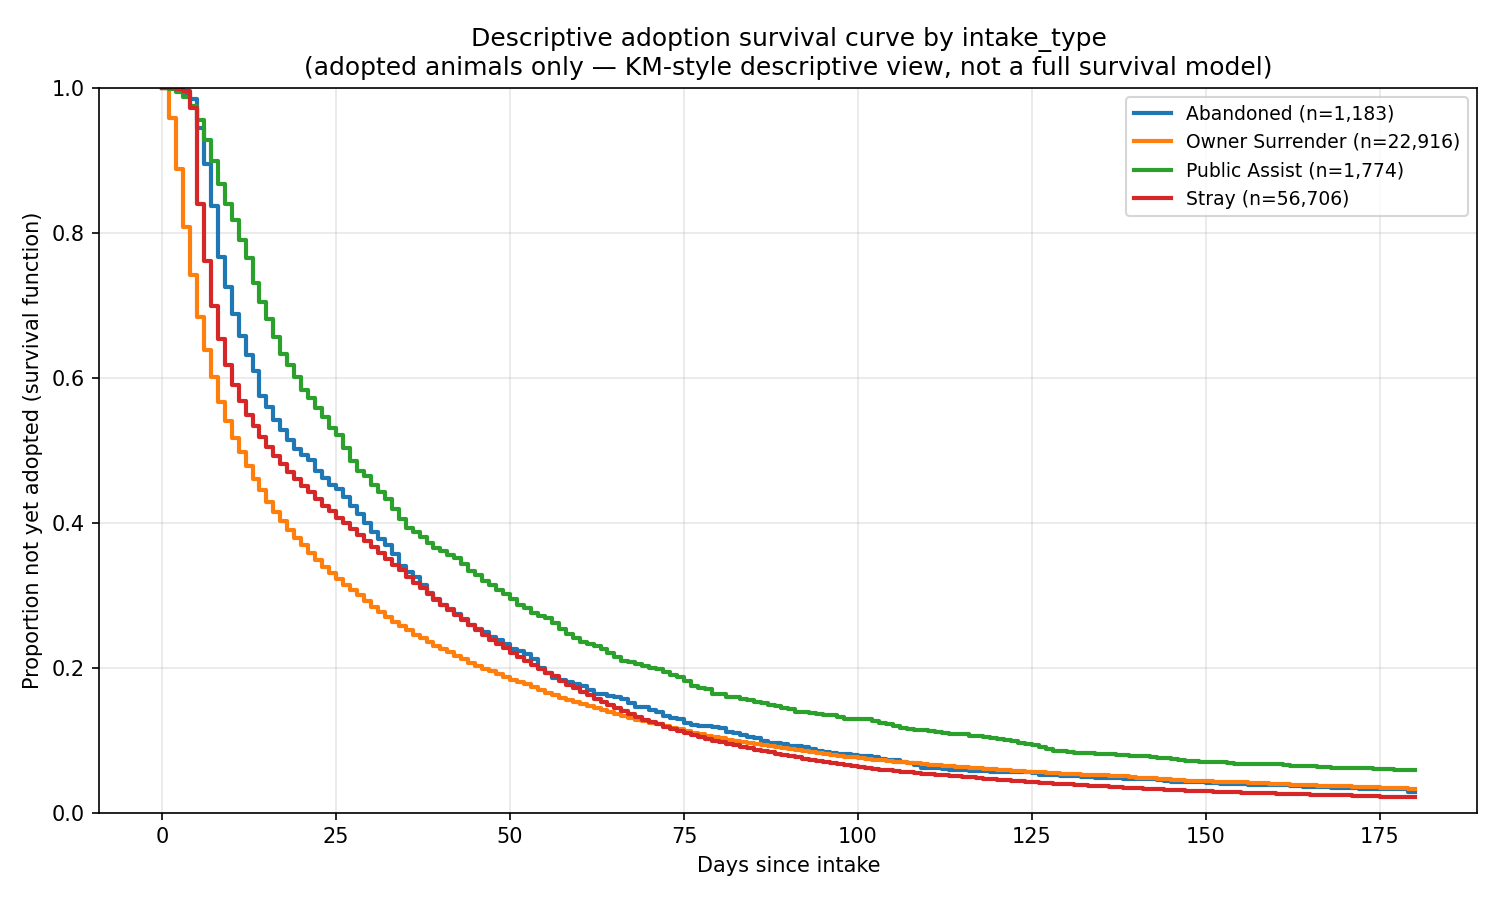
\includegraphics[width=0.92\textwidth]{../reports/figures/km_adoption_by_intake_type.png}
\caption{Krzywe Kaplana-Meiera czasu do adopcji według sposobu przyjęcia (wyłącznie adoptowane). Zwierzęta przyjęte w ramach zrzeczeń właścicielskich (\texttt{Owner Surrender}) trafiają do nowych domów szybciej niż bezpańskie (\texttt{Stray}).}
\label{fig:km_adoption_by_intake_type}
\end{figure}

Prawdopodobieństwo adopcji maleje wraz z wiekiem zwierzęcia. Grupa najmłodsza (\texttt{baby}) charakteryzuje się wskaźnikiem adopcji na poziomie 59,7\%, młodzież (\texttt{young}) --- 47,5\%, zwierzęta dorosłe (\texttt{adult}) --- 39,6\%, a starsze (\texttt{senior}) --- 31,0\%.

Sposób przyjęcia również wiąże się ze znaczną zmiennością wyników. Wśród 116 393 zwierząt znalezionych na ulicy (\texttt{Stray}) adopcją zakończyło się 48,7\% pobytów. Natomiast wśród 34 142 zrzeczeń właścicielskich (\texttt{Owner Surrender}) wskaźnik ten wyniósł 67,1\%.

\begin{figure}[htbp]
\centering
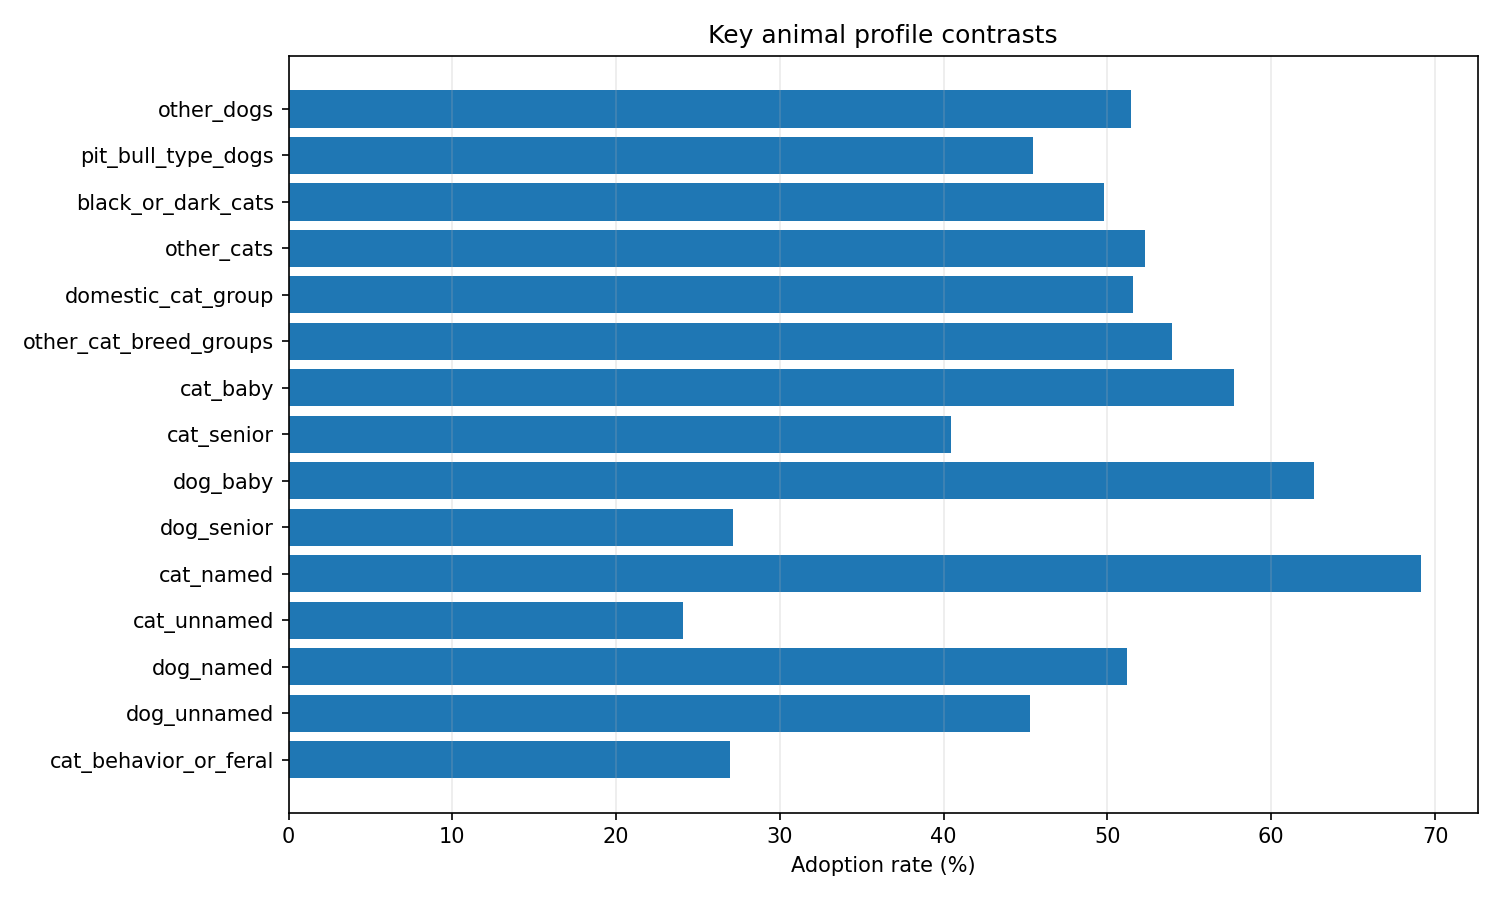
\includegraphics[width=0.92\textwidth]{../reports/figures/profile_contrasts_adoption_rate.png}
\caption{Porównanie wskaźników adopcji między typowymi profilami zwierząt.}
\label{fig:profile_contrasts}
\end{figure}

\section{Ograniczenia danych}
\label{sec:ograniczenia-danych}

Wykorzystany zbiór danych ma kilka ograniczeń.

Po pierwsze, pochodzi z placówki no-kill, czyli schroniska utrzymującego wysoki współczynnik uratowań i niestosującego rutynowej eutanazji zdrowych zwierząt \cite{Austin2010}. Wyniki mogą więc różnić się od wyników uzyskanych dla schronisk o innej specyfice działania.

Po drugie, wpisy dotyczące rasy i umaszczenia są deklaracją pracownika dokonaną przy przyjęciu, a nie wynikiem badań genetycznych. Etykiety takie jak \texttt{pit\_bull\_type} odzwierciedlają administracyjny sposób kategoryzacji psów oraz ludzką percepcję ich wyglądu.

Ograniczeniem technicznym było wykluczenie pobytów bez jednoznacznie zakończonego wyniku, co wynika z wymogu posiadania etykiety docelowej w nadzorowanym uczeniu maszynowym.

\section{Podsumowanie przygotowania danych}
\label{sec:podsumowanie-przygotowania-danych}

W wyniku opisanych przekształceń utworzono finalny zbiór modelowy obejmujący 162 390 epizodów pobytu psów i kotów w Austin Animal Center. Każdy rekord reprezentuje pojedyncze przyjęcie zwierzęcia, zestaw cech znanych w momencie tego przyjęcia oraz chronologicznie dopasowany wynik końcowy. Taka konstrukcja pozwala analizować proces pobytu z perspektywy informacji dostępnych przed rozstrzygnięciem sprawy zwierzęcia, a jednocześnie ogranicza ryzyko wycieku danych z przyszłości.

Najważniejszymi decyzjami przygotowawczymi były: ograniczenie populacji do psów i kotów, usunięcie rekordów bez podstawowych znaczników czasu i wyniku, dopasowanie przyjęć do najbliższych niewykorzystanych wyników oraz przekształcenie zmiennych opisowych do postaci możliwej do wykorzystania przez modele statystyczne. Szczególną uwagę zwrócono na zmienne, które mogą być dostępne dopiero po zakończeniu pobytu, ponieważ ich użycie prowadziłoby do sztucznego zawyżenia jakości predykcji.

Przygotowany zbiór stanowi podstawę dwóch zadań empirycznych rozwijanych w kolejnych rozdziałach: klasyfikacji prawdopodobieństwa adopcji oraz regresji długości pobytu do dowolnego dopasowanego wyniku. Rozdział następny opisuje metodykę modelowania, sposób podziału danych w czasie, dobór algorytmów oraz metryki użyte do oceny uzyskanych modeli.